\documentclass[conference]{IEEEtran}
\IEEEoverridecommandlockouts
% The preceding line is only needed to identify funding in the first footnote. If that is unneeded, please comment it out.
\usepackage{amsfonts,amsmath,amssymb,amstext,bm,cancel,dsfont,mathtools}
\usepackage{algorithm,algpseudocode,listings}
\usepackage{cite}
\usepackage{color,xcolor}
\usepackage{diagbox,tabularx}
\usepackage{enumerate}
\usepackage{epsfig,epstopdf,graphicx,multicol,multirow,palatino,pgfplots,tikz}
\usepackage{fancybox}
\usepackage{textcomp}
\usepackage{verbatim}

\def\BibTeX{{\rm B\kern-.05em{\sc i\kern-.025em b}\kern-.08em
    T\kern-.1667em\lower.7ex\hbox{E}\kern-.125emX}}

\graphicspath{{./Figure/}}
\epstopdfsetup{outdir=./Figure/Converted/}

% \floatname{algorithm}{Procedure}
\renewcommand{\algorithmicrequire}{\textbf{Input:}}
\renewcommand{\algorithmicensure}{\textbf{Output:}}

\pgfplotsset{compat=1.13}

% MATLAB
\lstset{extendedchars=false, basicstyle=\footnotesize\tt, language=Matlab, tabsize=4, numbers=left, numberstyle=\tiny, stepnumber=2, numbersep=4pt, keywordstyle=\color[rgb]{0,0,1}, commentstyle=\color[rgb]{0.133,0.545,0.133}, stringstyle=\color[rgb]{0.627,0.126,0.941}, backgroundcolor=\color{white}, showspaces=false, showstringspaces=false, showtabs=false, frame=false, captionpos=t, breaklines=true, breakatwhitespace=false, morekeywords={break, case, catch, continue, elseif, else, end, for, function, global, if, otherwise, persistent, return, switch, try, while}, title=\lstname,
mathescape=true,escapechar=? % escape to latex with ?..?  
escapeinside={\%*}{*)}, % if you want to add a comment within your code  
%morestring=[m]', % strings
%columns=fixed, % nice spacing
}

\begin{document}
\title{Implementation and Simulation of EKF-SLAM with Known and Unknown Correspondences in MATLAB\\ %and a Comparison to FastSLAM\\
% {\footnotesize \textsuperscript{*}Note: Sub-titles are not captured in Xplore and should not be used}
% \thanks{Identify applicable funding agency here. If none, delete this.}
}

\author{\IEEEauthorblockN{Sifan Jiang}
\IEEEauthorblockA{
% \textit{dept. name of organization (of Aff.)} \\
% \textit{name of organization (of Aff.)}\\
% City, Country \\
sifanj@kth.se
}
\and
\IEEEauthorblockN{Hongsheng Chang}
\IEEEauthorblockA{
% \textit{dept. name of organization (of Aff.)} \\
% \textit{name of organization (of Aff.)}\\
% City, Country \\
changh@kth.se
}
}
\maketitle

\begin{abstract}
This project is to implement 2-D extended Kalman filter Simultaneous Localization and Mapping (EKF-SLAM) and simulate the algorithm in the environment of MATLAB. The implementation would include both of the situations of known landmarks correspondences and unknown correspondences.
\end{abstract}

\begin{IEEEkeywords}
Data association, EKF-SLAM, MATLAB, SLAM
\end{IEEEkeywords}

%%%%%%%%%% ---------- %%%%%%%%%%
\section{Introduction}
\par For autonomous vehicles exploring unknown environments, the ability to perform Simultaneous Localization and Mapping is essential. The Simultaneous Localization and Mapping solves the problem of the incrementally building of the pose of a robot and the position of the landmarks when the robot is placed at an unknown location in an unknown environment which in another word is that the robot has to build a consistent map of the environment and simultaneously determine its pose based on this map \cite{EKF-SLAM-01}. The common process of SLAM requires a recursive procedure of prediction of the robot or vehicle's state based on the interior sensor or input control to move the target and correction of the state and map based on the observation data. The prediction step is straight forward while the correction step with unknown landmark correspondences includes data association problem and determining if an observation corresponds to a new landmark.
\par So far, there has been three main paradigms of the solution to the SLAM problem, which are SLAM based on Kalman filter and Particle filter, and Graph-based SLAM \cite{SLAM-01}. And in this project, EKF-SLAM would be implemented, which is a solution of the family of Kalman filter. Among various algorithms developed for solving SLAM problem, the EKF-SLAM remains on of the most popular ones and has been used for several practical applications. EKF-SLAM is a estimate method used for solving nonlinear system. Extended Kalman filter uses the first terms of Taylor expansion for linearize the motion model and observation model for making sure the noises at next timestamp is are Gaussian distributions as well. The main resource of the algorithm of the EKF-SLAM is from the book of \textit{Probabilistic Robotics} \cite{Probabilistic_Robotics}. Based on the algorithm and the code from \textit{Lab 1 of EL2320 Applied Estimation}, the EKF-SLAM in implemented and simulated in MATLAB.
\par Since the textbook of \textit{Probabilistic Robotics} only gives a pseudocode for the algorithm of EKF-SLAM, some part of the code is not so natural and even contradictory when coming to the MATLAB code which could cause the wrong size of matrix or even negative size of matrix \cite{Probabilistic_Robotics}. In this project, we implement an EKF-SLAM algorithm with unknown data association to avoid this situation from happening.
% \par Since SLAM is nonlinear estimation problem. When using EKF-SLAM algorithm, the estimates could tend to be inconsistent.
\par In all, the main contributions of this work are the  following: 
\begin{itemize}
	\item Implement 2-D EKF-SLAM algorithm in MATLAB and simulate the algorithm with map and sensor data from \textit{Lab files of EL2320 Applied Estimation}.
	\item Solve the data association problem of EKF-SLAM which is contradictory in the algorithm in the book of \textit{Probabilistic Robotics} \cite{Probabilistic_Robotics}.
	% \item Compare the EKF-SLAM to FastSLAM.
\end{itemize}

%%%%%%%%%% ---------- %%%%%%%%%%
\section{Simultaneous Localization and Mapping}
\par In probabilistic form, the Simultaneous Localization and Mapping problem could be described in \eqref{eq:probabilistic_SLAM}.
	\begin{align}
		P(\mathbf{x}_{k}, \mathbf{m} \;\vert\; \mathbf{Z}_{0:k}, \mathbf{U}_{0:k}, \mathbf{x}_{0})
		\label{eq:probabilistic_SLAM}
	\end{align}
Equation \eqref{eq:probabilistic_SLAM} describe the joint posterior density of the robot poses and landmark positions at timestamp $k$. To calculate the result of \eqref{eq:probabilistic_SLAM}, the Bayes filter is used. This computation requires a motion model and an observation model describing the effect of the control input and observation from the landmarks respectively \cite{SLAM-01}.
\par The motion model for the robot can be described as \eqref{eq:motion_model}.
	\begin{align}
		P(\mathbf{x}_{k} \;\vert\; \mathbf{x}_{k-1}, \mathbf{u}_{k}) \label{eq:motion_model}
	\end{align}
\par The observation model is to obtain the probability of making an observation $\mathbf{z}_{k}$ when the robot pose and landmark positions are known and can be described as \eqref{eq:observation_model}.
	\begin{align}
		P(\mathbf{z}_{k} \;\vert\; \mathbf{x}_{k}, \mathbf{m}) \label{eq:observation_model}
	\end{align}
\par Based on the motion model and the observation model, the SLAM algorithm is now implemented in Bayes filter, which is a recursive filter with prediction and correction steps:
	\begin{itemize}
		\item Prediction:
			\begin{align}
				& P(\mathbf{x}_{k}, \mathbf{m} \;\vert\; \mathbf{Z}_{0:k-1}, \mathbf{U}_{0:k}, \mathbf{x}_{0}) \nonumber \\
				= & \int P(\mathbf{x}_{k} \;\vert\; \mathbf{x}_{k-1}, \mathbf{u}_{k}) \nonumber \\
				& \times P(\mathbf{x}_{k-1}, \mathbf{m} \;\vert\; \mathbf{Z}_{0:k-1}, \mathbf{U}_{0:k-1}, \mathbf{x}_{0}) \mathrm{d}\mathbf{x}_{k-1} \label{eq:prediction}
			\end{align}
		\item Correction:
			\begin{align}
				& P(\mathbf{x}_{k}, \mathbf{m} \;\vert\; \mathbf{Z}_{0:k}, \mathbf{U}_{0:k}, \mathbf{x}_{0}) \nonumber \\
				= & \frac{P(\mathbf{z}_{k} \;\vert\; \mathbf{x}_{k}, \mathbf{m})P(\mathbf{x}_{k}, \mathbf{m} \;\vert\; \mathbf{Z}_{0:k-1}, \mathbf{U}_{0:k}, \mathbf{x}_{0})}{P(\mathbf{z}_{k} \;\vert\; \mathbf{Z}_{0:k-1}, \mathbf{U}_{0:k})} \label{eq:correction}
			\end{align}
	\end{itemize}
\par The whole procedure of SLAM is illustrated in Fig.~\ref{fig:SLAM}.
	\begin{figure}[htbp]
		\centering
		\includegraphics[width=0.45\textwidth]{SLAM.png}
		\caption{SLAM Problem}
		\label{fig:SLAM}
	\end{figure}

%%%%%%%%%% ---------- %%%%%%%%%%
\section{EKF-SLAM Algorithms in \textit{Probabilistic Robotics}}
\par In EKF-SLAM, the motion model is changed from \eqref{eq:motion_model} to \eqref{eq:EKF_motion_model} and the observation model is changed from \eqref{eq:observation_model} to \eqref{eq:EKF_observation_model}.
	\begin{align}
		P(\mathbf{x}_{k} \;\vert\; \mathbf{x}_{k-1}, \mathbf{u}_{k}) & \Longleftrightarrow \mathbf{x}_{k} = \mathbf{g}(\mathbf{x}_{k-1}, \mathbf{u}_{t}) + \mathbf{w}_{k} \label{eq:EKF_motion_model} \\
		P(\mathbf{z}_{k} \;\vert\; \mathbf{x}_{k}, \mathbf{m}) & \Longleftrightarrow \mathbf{z}(k) = \mathbf{h}(\mathbf{x}_{k}, \mathbf{m}) + \mathbf{v}_{k} \label{eq:EKF_observation_model}
	\end{align}
where $\mathbf{g}(\cdot)$ describes the vehicle kinematics and $\mathbf{h}(\cdot)$ describes the geometry of the observation. Also $\mathbf{w}_{k}$ and $\mathbf{v}_{k}$ are additive, zero mean uncorrelated Gaussian motion disturbances with covariance $\mathbf{Q}_{k}$ and observation errors with covariance $\mathbf{R}_{k}$ respectively \cite{EKF-SLAM-02}.
\par The vector space of state in 2-D condition at timestamp $k$ is $\bm{\mu}_{k} = \left[x \; y \; \theta \; m_{1,x} \; m_{1,y} \; \cdots \; m_{N,x} \; m_{N,y} \right]^{T}$ where $x$, $y$, and $\theta$ refer to $x$-coordinate, $y$-coordinate, and orientation (heading angle) of the robot and $m_{j,x}$, and $m_{j,y}$ are the position of $j$-th landmark. In abbreviation, $\bm{\mu}_{k} = \left[ \mathbf{X} \; \mathbf{M} \right]^{T}$.
\par The covariance matrix of the state vector at timestamp $k$ in abbreviation would be
$$
\bm{\Sigma}_{k} = \begin{pmatrix}
\mathbf{\Sigma}_{\mathbf{X}\mathbf{X}} & \mathbf{\Sigma}_{\mathbf{X}\mathbf{M}} \\
\mathbf{\Sigma}_{\mathbf{M}\mathbf{X}} & \mathbf{\Sigma}_{\mathbf{M}\mathbf{M}}
\end{pmatrix}
$$
\par The initial state and covariance are set to be $\bm{\mu}_{0} = \left[0 \; 0 \; 0 \; 0 \; \cdots \; 0 \right]^{T}$ and
$$
\bm{\Sigma}_{0} = \begin{pmatrix}
0 		& 0 	 & 0 	  & 0 	   & \cdots & 0 	 \\
0 		& 0 	 & 0 	  & 0 	   & \cdots & 0 	 \\
0 		& 0 	 & 0 	  & 0 	   & \cdots & 0 	 \\
0 		& 0 	 & 0 	  & \infty & \cdots & 0 	 \\
\vdots 	& \vdots & \vdots & \vdots & \ddots & \vdots \\
0 		& 0 	 & 0 	  &	0 	   & \cdots	& \infty
\end{pmatrix}
$$
When data association is unknown, we also need to initialize the number of landmarks to $N_{0}=0$. In both cases (known and unknown data association), a newly observed landmark need to be initialize (set position based on the observation and robot pose).
\par The EKF-SLAM Algorithm with known data association in \cite{Probabilistic_Robotics} is shown in Alg.~\ref{alg:EKF_SLAM_Known_Correspondences}. The EKF-SLAM Algorithm with unknown data association in \cite{Probabilistic_Robotics} is shown in Alg.~\ref{alg:EKF_SLAM_Unknown_Correspondences}. The algorithm is mainly follow the book, however, at some minor change is applied for convenient implementation in MATLAB. The lines 17 and 18 in known data association case and lines 21 and 22 in unknown data assocation case is added for reducing the memory consumption.
\begin{algorithm}[htbp]
	\caption{EKF\_SLAM\_Known\_Correspondences}
	\label{alg:EKF_SLAM_Known_Correspondences}
	\scriptsize
	\begin{algorithmic}[1]
		\Require $\mu_{t-1}$, $\Sigma_{t-1}$, $u_{t}$, $z_{t}$, $c_{t}$
		\State $F_{x} = \begin{pmatrix} 1 & 0 & 0 & 0 \cdots 0 \\ 0 & 1 & 0 & 0 \cdots 0 \\ 0 & 0 & 1 & \underbrace{0 \cdots 0}_{2N} \end{pmatrix}$
		\State $\bar{\mu}_{t} = \mu_{t-1} + F_{x}^{T} \begin{pmatrix} -\frac{v_{t}}{\omega_{t}}\sin{\mu_{t-1,\theta}} + \frac{v_{t}}{\omega_{t}}\sin(\mu_{t-1,\theta}+\omega_{t}\Delta{t}) \\ \frac{v_{t}}{\omega_{t}}\cos{\mu_{t-1,\theta}} - \frac{v_{t}}{\omega_{t}}\cos(\mu_{t-1,\theta}+\omega_{t}\Delta{t}) \\ \omega_{t}\Delta{t} \end{pmatrix}$
		\State $G_{t} = I + F_{x}^{T} \begin{pmatrix} 0 & 0 & \frac{v_{t}}{\omega_{t}}\cos{\mu_{t-1,\theta}} - \frac{v_{t}}{\omega_{t}}\cos(\mu_{t-1,\theta}+\omega_{t}\Delta{t}) \\ 0 & 0 & \frac{v_{t}}{\omega_{t}}\sin{\mu_{t-1,\theta}} - \frac{v_{t}}{\omega_{t}}\sin(\mu_{t-1,\theta}+\omega_{t}\Delta{t}) \\ 0 & 0 & 0 \end{pmatrix} F_{x}$
		\State $\bar{\Sigma}_{t} = G_{t}\Sigma_{t-1}G_{t}^{T} + F_{x}^{T}R_{t}F_{x}$
		\State $Q_{t} = \begin{pmatrix} \sigma_{r} & 0 \\ 0 & \sigma_{\phi} \end{pmatrix}$
		\For{All Observed Features $z_{t}^{i} = (r_{t}^{i} \; \phi_{t}^{i})$}
			\State $j = c_{t}^{i}$ \Comment{$c_{t}^{i}$ is the known correspondence}
			\If{Landmark $j$ never seen before}
				\State $\begin{pmatrix} \bar{\mu}_{j,x} \\ \bar{\mu}_{j,y} \end{pmatrix} = \begin{pmatrix} \bar{\mu}_{t,x} \\ \bar{\mu}_{t,y} \end{pmatrix} + r_{t}^{i}\begin{pmatrix} \cos(\phi_{t}^{i}+\mu_{t,\theta}) \\ \sin(\phi_{t}^{i}+\mu_{t,\theta}) \end{pmatrix}$
			\EndIf
			\State $\delta = \begin{pmatrix} \delta_{x} \\ \delta_{y} \end{pmatrix} = \begin{pmatrix} \bar{\mu}_{j,x}-\bar{\mu}_{t,x} \\ \bar{\mu}_{j,y}-\bar{\mu}_{t,y} \end{pmatrix}$
			\State $q = \delta^{T}\delta$
			\State $\hat{z}_{t}^{i} = \begin{pmatrix} \sqrt{q} \\ \mathrm{atan2}(\delta_{y},\delta_{x})-\bar{\mu}_{t,\theta} \end{pmatrix}$
			\State $F_{x,j} = \begin{pmatrix} 1 & 0 & 0 & 0 \cdots 0 & 0 & 0 & 0 \cdots 0 \\ 0 & 1 & 0 & 0 \cdots 0 & 0 & 0 & 0 \cdots 0 \\ 0 & 0 & 1 & 0 \cdots 0 & 0 & 0 & 0 \cdots 0 \\ 0 & 0 & 0 & 0 \cdots 0 & 1 & 0 & 0 \cdots 0 \\ 0 & 0 & 0 & \underbrace{0 \cdots 0}_{2j-2} & 0 & 1 & \underbrace{0 \cdots 0}_{2N-2j} \end{pmatrix}$
			\State $H_{t}^{i} = \frac{1}{q} \begin{pmatrix} \sqrt{q}\delta_{x} & -\sqrt{q}\delta_{y} & 0 & -\sqrt{q}\delta_{x} & \sqrt{q}\delta_{y} \\ \delta_{y} & \delta_{x} & -1 & -\delta_{y} & -\delta_{x} \end{pmatrix} F_{x,j}$
			\State $K_{t}^{i} = \hat{\Sigma}_{t}{H_{t}^{i}}^{T}(H_{t}^{i}\hat{\Sigma}_{t}{H_{t}^{i}}^{T} + Q_{t})^{-1}$
			\State $\bar{\mu}_{t} = \bar{\mu}_{t} + K_{t}^{i}(z_{t}^{i} - \hat{z}_{t}^{i})$
			\State $\bar{\Sigma}_{t} = (I-K_{t}^{i}H_{t}^{i})\bar{\Sigma}_{t}$
		\EndFor
		\State $\mu_{t} = \bar{\mu}_{t}$
		\State $\Sigma_{t} = \bar{\Sigma}_{t}$
		\Ensure $\mu_{t}$, $\Sigma_{t}$
	\end{algorithmic}
\end{algorithm}

\begin{algorithm}[htbp]
	\caption{EKF\_SLAM\_Unknown\_Correspondences}
	\label{alg:EKF_SLAM_Unknown_Correspondences}
	\scriptsize
	\begin{algorithmic}[1]
		\Require $\mu_{t-1}$, $\Sigma_{t-1}$, $u_{t}$, $z_{t}$, $N_{t-1}$
		\State $F_{x} = \begin{pmatrix} 1 & 0 & 0 & 0 \cdots 0 \\ 0 & 1 & 0 & 0 \cdots 0 \\ 0 & 0 & 1 & 0 \cdots 0 \end{pmatrix}$
		\State $\bar{\mu}_{t} = \mu_{t-1} + F_{x}^{T} \begin{pmatrix} -\frac{v_{t}}{\omega_{t}}\sin{\mu_{t-1,\theta}} + \frac{v_{t}}{\omega_{t}}\sin(\mu_{t-1,\theta}+\omega_{t}\Delta{t}) \\ \frac{v_{t}}{\omega_{t}}\cos{\mu_{t-1,\theta}} - \frac{v_{t}}{\omega_{t}}\cos(\mu_{t-1,\theta}+\omega_{t}\Delta{t}) \\ \omega_{t}\Delta{t} \end{pmatrix}$
		\State $G_{t} = I + F_{x}^{T} \begin{pmatrix} 0 & 0 & \frac{v_{t}}{\omega_{t}}\cos{\mu_{t-1,\theta}} - \frac{v_{t}}{\omega_{t}}\cos(\mu_{t-1,\theta}+\omega_{t}\Delta{t}) \\ 0 & 0 & \frac{v_{t}}{\omega_{t}}\sin{\mu_{t-1,\theta}} - \frac{v_{t}}{\omega_{t}}\sin(\mu_{t-1,\theta}+\omega_{t}\Delta{t}) \\ 0 & 0 & 0 \end{pmatrix} F_{x}$
		\State $\bar{\Sigma}_{t} = G_{t}\Sigma_{t-1}G_{t}^{T} + F_{x}^{T}R_{t}F_{x}$
		\State $Q_{t} = \begin{pmatrix} \sigma_{r} & 0 \\ 0 & \sigma_{\phi} \end{pmatrix}$
		\For{All Observed Features $z_{t}^{i} = (r_{t}^{i} \; \phi_{t}^{i})$}
			\State $\begin{pmatrix} \bar{\mu}_{N_{t}+1,x} \\ \bar{\mu}_{N_{t}+1,y} \end{pmatrix} = \begin{pmatrix} \bar{\mu}_{t,x} \\ \bar{\mu}_{t,y} \end{pmatrix} + r_{t}^{i} \begin{pmatrix} \cos(\phi_{t}^{i}+\bar{\mu}_{t,\theta}) \\ \sin(\phi_{t}^{i}+\bar{\mu}_{t,\theta}) \end{pmatrix}	$
			\For{$k=1 \; \mathrm{\textbf{to}} \; N_{t}+1$} % !!!!!
				\State $\delta_{k} = \begin{pmatrix} \delta_{k,x} \\ \delta_{k,y} \end{pmatrix} = \begin{pmatrix} \bar{\mu}_{k,x}-\bar{\mu}_{t,x} \\ \bar{\mu}_{k,y}-\bar{\mu}_{t,y} \end{pmatrix}$
				\State $q_{k} = \delta_{k}^{T}\delta_{k}$
				\State $\hat{z}_{t}^{k} = \begin{pmatrix} \sqrt{q_{k}} \\ \mathrm{atan2}(\delta_{k,y},\delta_{k,x})-\bar{\mu}_{t,\theta} \end{pmatrix}$
				\State $F_{x,k} = \begin{pmatrix} 1 & 0 & 0 & 0 \cdots 0 & 0 & 0 & 0 \cdots 0 \\ 0 & 1 & 0 & 0 \cdots 0 & 0 & 0 & 0 \cdots 0 \\ 0 & 0 & 1 & 0 \cdots 0 & 0 & 0 & 0 \cdots 0 \\ 0 & 0 & 0 & 0 \cdots 0 & 1 & 0 & 0 \cdots 0 \\ 0 & 0 & 0 & 0 \cdots 0 & 0 & 1 & 0 \cdots 0 \end{pmatrix}$
				{\tiny\State $H_{t}^{k} = \frac{1}{q_{k}} \begin{pmatrix} \sqrt{q_{k}}\delta_{k,x} & -\sqrt{q_{k}}\delta_{k,y} & 0 & -\sqrt{q_{k}}\delta_{k,x} & \sqrt{q_{k}}\delta_{k,y} \\ \delta_{k,y} & \delta_{k,x} & -1 & -\delta_{k,y} & -\delta_{k,x}  \end{pmatrix} F_{x,k}$}
				\State $\Psi_{k} = H_{t}^{k}\bar{\Sigma}_{t}{H_{t}^{k}}^{T} + Q_{t}$
				\State $\pi_{k} = (z_{t}^{i}-\hat{z}_{t}^{k})^{T} \Psi_{k}^{-1} (z_{t}^{i}-\hat{z}_{t}^{k})$
			\EndFor
			\State $\pi_{N_{t}+1} = \alpha$
			\State $j(i) = \mathrm{argmin}_{k} \; \pi_{k}$
			\State $N_{t} = \mathrm{max}\{N_{t},j(i)\}$
			\State $K_{t}^{i} = \hat{\Sigma}_{t}[{H_{t}^{j(i)}}]^{T}\Psi_{j(i)}^{-1}$
			\State $\bar{\mu}_{t} = \bar{\mu}_{t} + K_{t}^{i}(z_{t}^{i} - \hat{z}_{t}^{j(i)})$
			\State $\bar{\Sigma}_{t} = (I-K_{t}^{i}H_{t}^{j(i)})\bar{\Sigma}_{t}$
		\EndFor
		\State $\mu_{t} = \bar{\mu}_{t}$
		\State $\Sigma_{t} = \bar{\Sigma}_{t}$
		\Ensure $\mu_{t}$, $\Sigma_{t}$, $N_{t}$
	\end{algorithmic}
\end{algorithm}
\par In both of the algorithms for known or unknown data association, the procedure before the first \textbf{For} loop is the prediction step and the procedure in the \textbf{For} loop is correction step. The algorithm in the textbook gives a detailed way to calculate the odometry of the robot which would be simplified in the implementation. Matrix $F_{x}$ is used for matching the dimension difference between two matrix. In known correspondences case, since we assume the number of landmarks is also known, the main problem and difference from EKF localization is the initialization of newly observed landmark. To determine if the landmark observed has never been seen before is simple, a state vector for all the landmarks could be created to store such information which would be illustrated in following part. To initialize the landmark, the position of the landmark can be calculated by pose of the robot and the observation to such landmark which is a simple problem of geometry.
\par In the case of unknown data association, since the number and signature of the landmarks remains unknown, the main problem would also be determining if an observed landmark is a new landmark or not. In the textbook, the observed landmark would always be assumed as a new landmark at first. If the Mahalanobis distance of all existing landmarks in the map exceeds the threshold (value $\alpha$), the landmark then would be considered as a new one. Since the signature of landmarks is unknown, for each newly observed landmarks, the signature of it would be determined sequentially. Also the matrix size in the unknown correspondences case is tricky.

%%%%%%%%%% ---------- %%%%%%%%%%
\section{Implementation and Simulation of 2-D EKF-SLAM in MATLAB}
	%%%%% ----- %%%%%
\subsection{Implementation}
\par The main structure of our implementation is based on the programme from the \textit{Lab files of EL2320 Applied Estimation} to give realize the reading and segmenting data from text files into different MATLAB variables. Also, we use some tool functions which were created by \textit{Kai Arras} from \textit{CAS-KTH} to plot the state of robot with covariance based ellipse to create gif videos. For the algorithm part of the code, in both cases it is divided into two parts: \texttt{predict.m} and \texttt{correct.m}.
\par As mentioned above, the motion model of the robot is simplied in the implementation, thus the prediction part would be changed into \eqref{eq:simplified_motion} and \eqref{eq:simplified_motion_Jacobian}.
	\begin{align}
		\bar{\mu}_{t} & = \mu_{t-1} + F_{x}^{T} \begin{pmatrix} v_{t}\Delta{t}\cos{\mu_{t-1,\theta}} \\ v_{t}\Delta{t}\sin{\mu_{t-1,\theta}} \\ \omega_{t}\Delta{t} \end{pmatrix} \label{eq:simplified_motion} \\
		G_{t} & = I + F_{x}^{T} \begin{pmatrix} 0 & 0 & -v_{t}\Delta{t}\sin{\mu_{t-1,\theta}} \\ 0 & 0 & v_{t}\Delta{t}\cos{\mu_{t-1,\theta}} \\ 0 & 0 & 0 \end{pmatrix} F_{x} \nonumber \\
		& = I + F_{x}^{T} \begin{pmatrix} 0 & 0 & -\bar{\mu}_{t,y} \\ 0 & 0 & \bar{\mu}_{t,x} \\ 0 & 0 & 0 \end{pmatrix} F_{x} \label{eq:simplified_motion_Jacobian}
	\end{align}
% \lstinputlisting{predict.m}
		%% -- %%
\subsubsection{Known Data Association}
\par As mentioned above, one of the problem of SLAM is to determine whether an observed landmark has never been seen before. In known data association case, a matrix \texttt{landmark\_obs\_flag} is used for recording the observation state of the landmarks.
% \lstinputlisting{correct_known.m}
		%% -- %%
\subsubsection{Unknown Data Association}
\par The main problem of the during the implementaion of EKF-SLAM with unknown data association is in the \textbf{For} loop of line 8 in Alg.~\ref{alg:EKF_SLAM_Unknown_Correspondences}. When $k=N_{t}+1$, $2N_{t}-2k=-2$ which is the width of zeros in matrix $F_{x,k}$ and should never be negative. And the reason why the size of the matrix is in such number is to match the size of $\bar{\Sigma}_{t}$ obtained from the predict step which would be naturally be of size $(2N_{t}+3)\times(2N_{t}+3)$.
\par The solution in the implementation is to expand the size of $\bar{\Sigma}_{t}$ before the \textbf{For} loop of line 8 in Alg.~\ref{alg:EKF_SLAM_Unknown_Correspondences}, such that
	\begin{align*}
		\bar{\Sigma}_{t} = \begin{pmatrix} \bar{\Sigma}_{t} & \mathbf{0}^{T} \\ \mathbf{0} & \bm{\infty} \end{pmatrix}
	\end{align*}
where
	\begin{align*}
		\mathbf{0} & = \begin{pmatrix} 0 \; \cdots \; 0 \\ \underbrace{0 \; \cdots \; 0}_{2N_{t}+3} \end{pmatrix} \\
		\bm{\infty} & = \begin{pmatrix} \infty & 0 \\ 0 & \infty \end{pmatrix}
	\end{align*}
\par The size of $\Sigma$ at this moment is $[2(N_{t}+1)+3]\times[2(N_{t}+1)+3]$. If the observed landmark is not a new landmark, then
	$$ \bar{\Sigma}_{t} = \bar{\Sigma}_{t}\left( 1:(2N_{t}+3), 1:(2N_{t}+3) \right)$$
\par Futhermore, the number of zeros in matrix $F_{x,k}$ would be changed to $2(N_{t}+1)-2k$, thus the value would always be bigger or equal to zero.
% \lstinputlisting{correct_unknown.m}
	%%%%% ----- %%%%%
\subsection{Experimental Results}
\par The simulation of EKF-SLAM is shown in videos and can be found under Video folder.
		%% -- %%
\subsubsection{Known Data Association}
	\begin{itemize}
		\item \texttt{map\_o3.txt} + \texttt{so\_o3\_ie.txt}:
			\par According to the description of \textit{Lab 1 of EL2320 Applied Estimation}, the laser scanner has an accuracy of (1 cm, 1 degree), the odometry information has an un-modeled noise of approximately 1 cm and 1 degree per time step. So the motion distrubance and observation noise are set to be
				\begin{align*}
					R & = \begin{pmatrix} 0.01^2 & 0 & 0 \\ 0 & 0.01^2 & 0 \\ 0 & 0 & (2\pi / 360)^2 \end{pmatrix} \\
					Q & = \begin{pmatrix} 0.01^2 & 0 \\ 0 & (2\pi/360)^2 \end{pmatrix}
				\end{align*}
			\par The simulation result is shown in Fig.~\ref{fig:map_o3+so_o3_ie+Trace}, \ref{fig:map_o3+so_o3_ie+Error}, and \ref{fig:map_o3+so_o3_ie+Variance}, and video \texttt{map\_o3+Video.gif}.
				\begin{figure}[htbp]
					\centering
					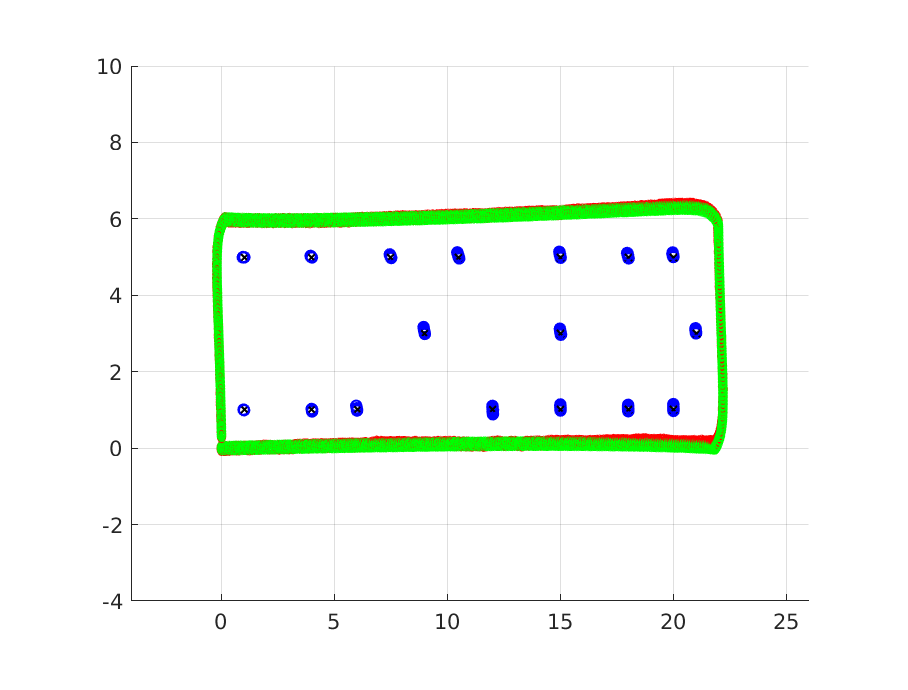
\includegraphics[width=0.45\textwidth]{map_o3+so_o3_ie+Trace.eps}
					\caption{Trace of Robot Pose and Map Location}
					\label{fig:map_o3+so_o3_ie+Trace}
				\end{figure}
				\begin{figure}[htbp]
					\centering
					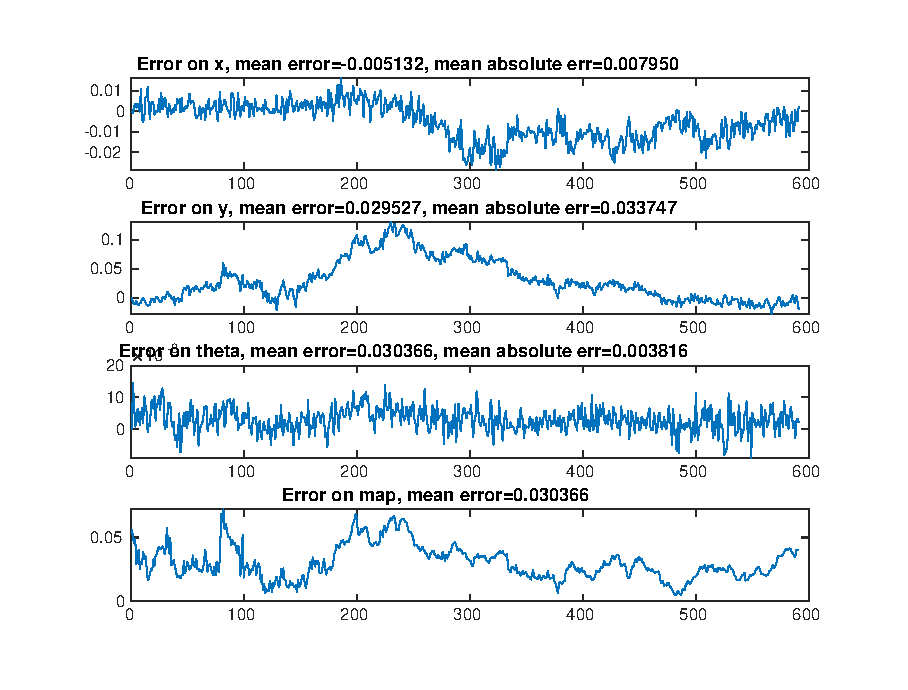
\includegraphics[width=0.45\textwidth]{map_o3+so_o3_ie+Error.eps}
					\caption{Error of Robot Pose and Average Map Location}
					\label{fig:map_o3+so_o3_ie+Error}
				\end{figure}
				\begin{figure}[htbp]
					\centering
					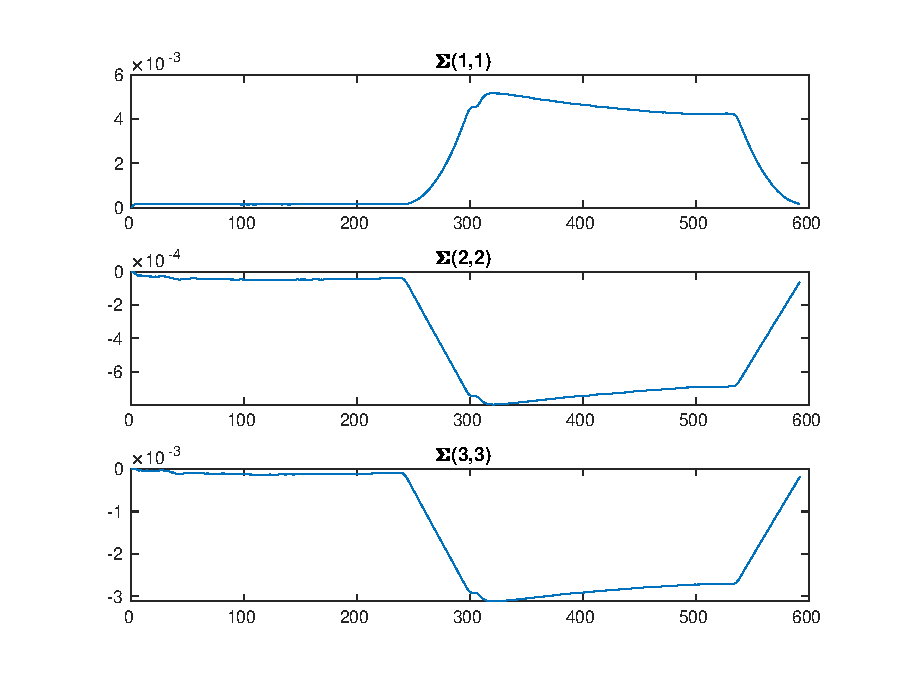
\includegraphics[width=0.45\textwidth]{map_o3+so_o3_ie+Variance.eps}
					\caption{Variance of Robot Pose}
					\label{fig:map_o3+so_o3_ie+Variance}
				\end{figure}
			\par As shown in the figures, the estimation of robot pose and landmark position is relatively close to the true pose of robot and landmarks. The error or the robot pose and average position of landmarks are small. Also, the covariance of the robot pose is small. Overall, the EKF-SLAM conducts well performance on this data sets.
		\item \texttt{map\_pent\_big\_40.txt} + \texttt{so\_pb\_40\_no.txt}:
			\par According to the description, the measurement noise is modeled with a standard deviation of 0.1 (m, rad) and the process noise is modeled with a standard deviation of 1 (m, m, rad). Also, the shape of the map should be noticed that the landmarks form a circle with is highly symmetric. So that the distrubance and noise are
				\begin{align*}
					R & = \begin{pmatrix} 1 & 0 & 0 \\ 0 & 1 & 0 \\ 0 & 0 & 1 \end{pmatrix} \\
					Q & = \begin{pmatrix} 0.1 & 0 \\ 0 & 0.1 \end{pmatrix}
				\end{align*}
			\par The result is shown in Fig.~\ref{fig:map_pent_big_40+Trace}, \ref{fig:map_pent_big_40+Error}, and \ref{fig:map_pent_big_40+Variance}.
				\begin{figure}[htbp]
					\centering
					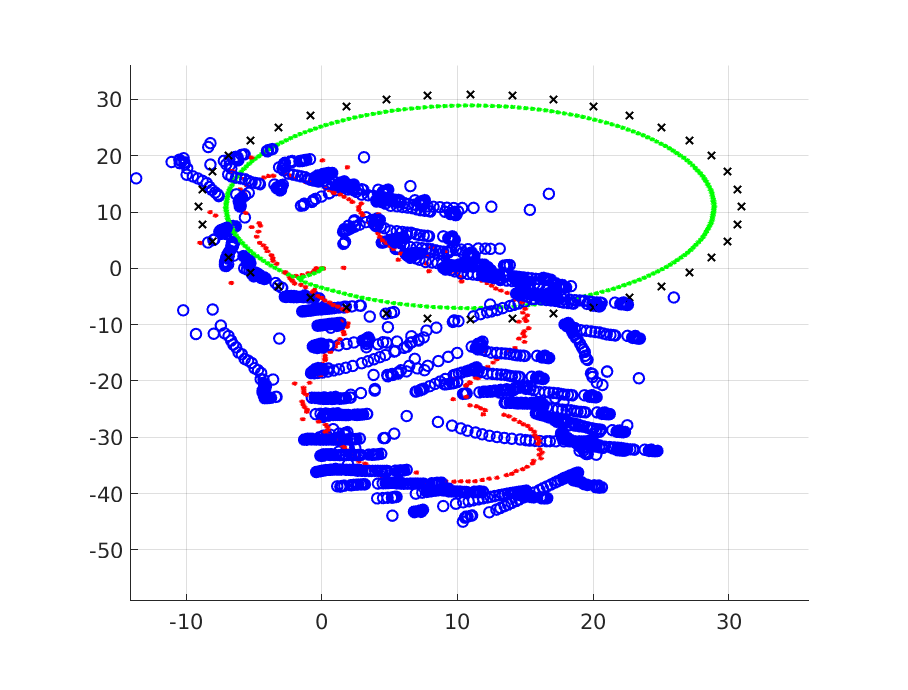
\includegraphics[width=0.45\textwidth]{map_pent_big_40+Trace.eps}
					\caption{Trace of Robot Pose and Map Location}
					\label{fig:map_pent_big_40+Trace}
				\end{figure}
				\begin{figure}[htbp]
					\centering
					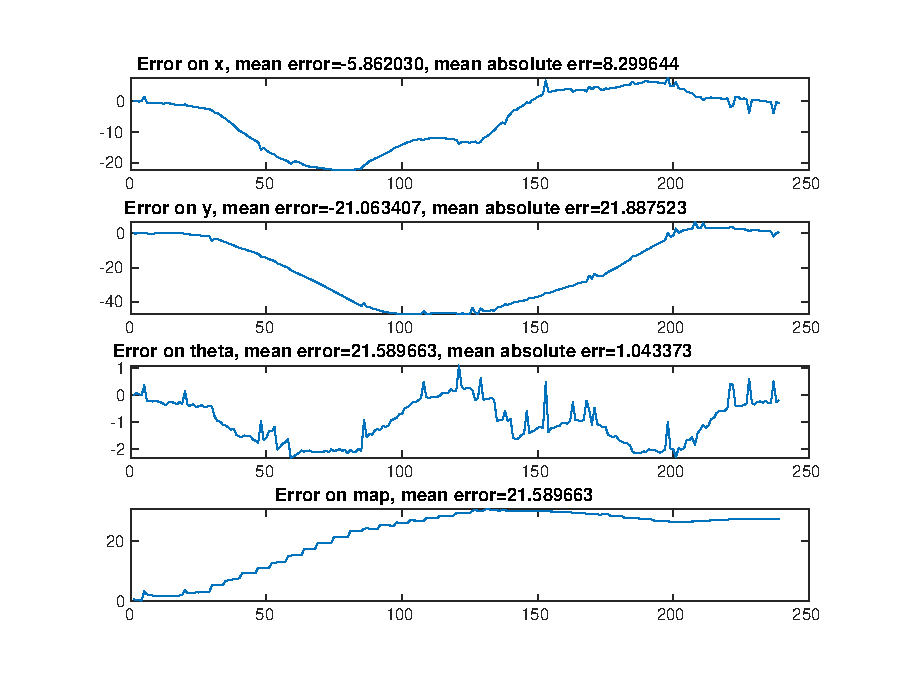
\includegraphics[width=0.45\textwidth]{map_pent_big_40+Error.eps}
					\caption{Error of Robot Pose and Average Map Location}
					\label{fig:map_pent_big_40+Error}
				\end{figure}
				\begin{figure}[htbp]
					\centering
					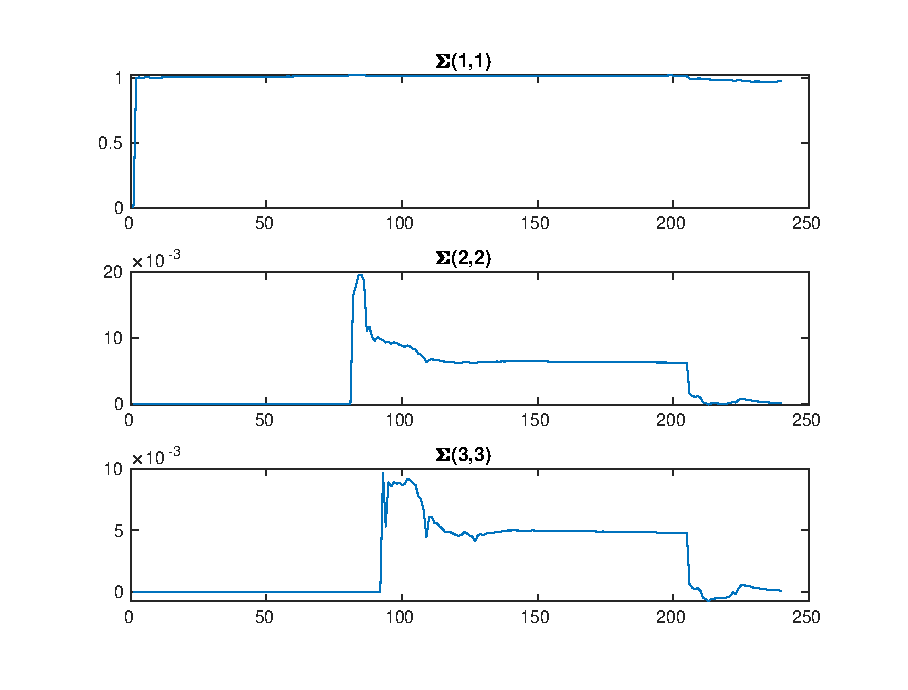
\includegraphics[width=0.45\textwidth]{map_pent_big_40+Variance.eps}
					\caption{Error of Robot Pose and Average Map Location}
					\label{fig:map_pent_big_40+Variance}
				\end{figure}
			\par As shown in the figures, the EKF-SLAM has bad performance on this data sets with totally wrong estimation of robot poses and landmarks positions. The reason could be:
				\begin{itemize}
					\item The observation data of this data set could contain outliers. Unlike localization problems which can detect outliers based on the position of the landmarks to calculate Mahalanobis distances and use threshold to determine whether this observation is a outlier or not, the SLAM problem can not determine outlier since the observation may find a new landmark.
					\item Since the SLAM problem often includes highly non-linear motion for the robot, thus extended Kalman filter could give wrong and inconsistent prediction for the pose and position.
				\end{itemize}
	\end{itemize}
		%% -- %%
\subsubsection{Unknown Data Association}
\par Still, test on two data sets which are same to the case of known data association, and the setting of the motion disturbance and observation noise are same to the above case.
	\begin{itemize}
		\item \texttt{map\_o3.txt} + \texttt{so\_o3\_ie.txt}:
			\par The result is illustrated in Fig.~\ref{fig:map_o3+Unknown+Trace}, \ref{fig:map_o3+Unknown+Error}, and \ref{fig:map_o3+Unknown+Variance}.
				\begin{figure}[htbp]
					\centering
					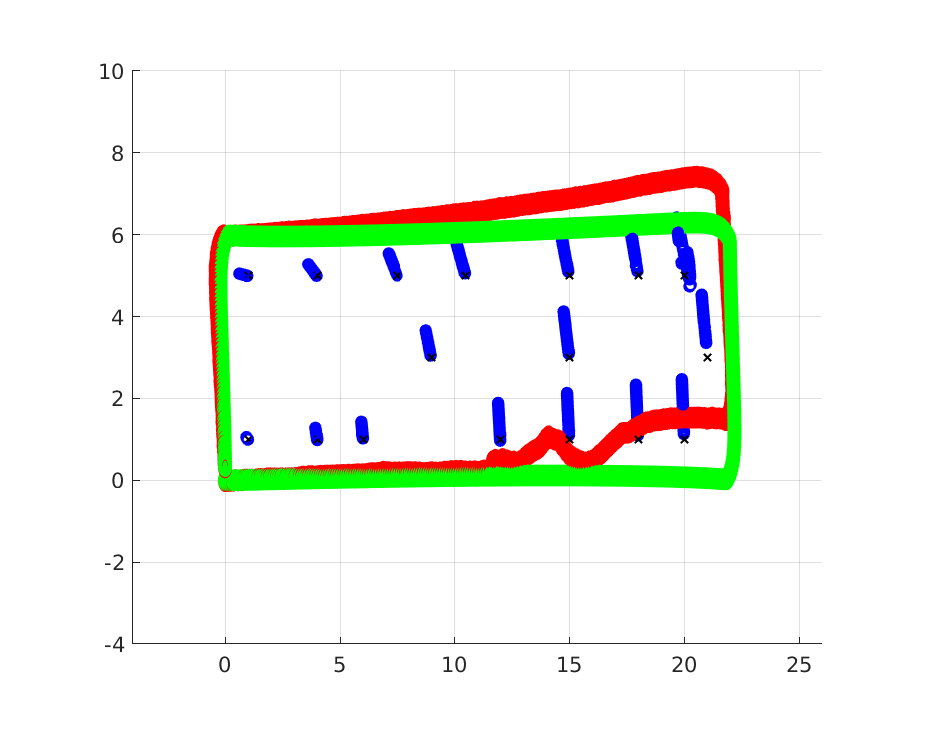
\includegraphics[width=0.45\textwidth]{map_o3+Unknown+Trace.eps}
					\caption{Trace of Robot Pose and Map Location}
					\label{fig:map_o3+Unknown+Trace}
				\end{figure}
				\begin{figure}[htbp]
					\centering
					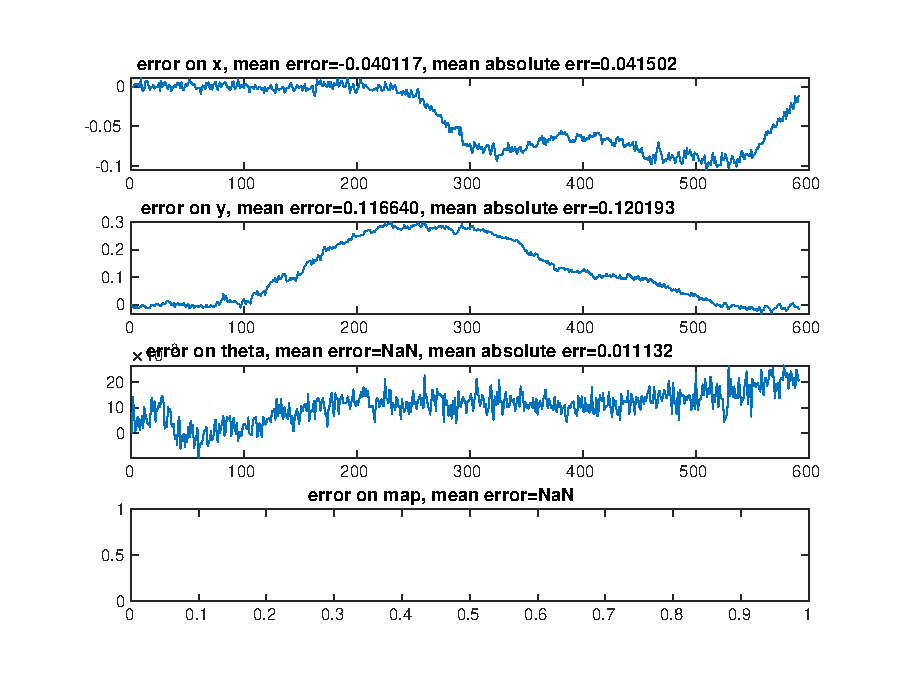
\includegraphics[width=0.45\textwidth]{map_o3+Unknown+Error.eps}
					\caption{Error of Robot Pose and Average Map Location}
					\label{fig:map_o3+Unknown+Error}
				\end{figure}
				\begin{figure}[htbp]
					\centering
					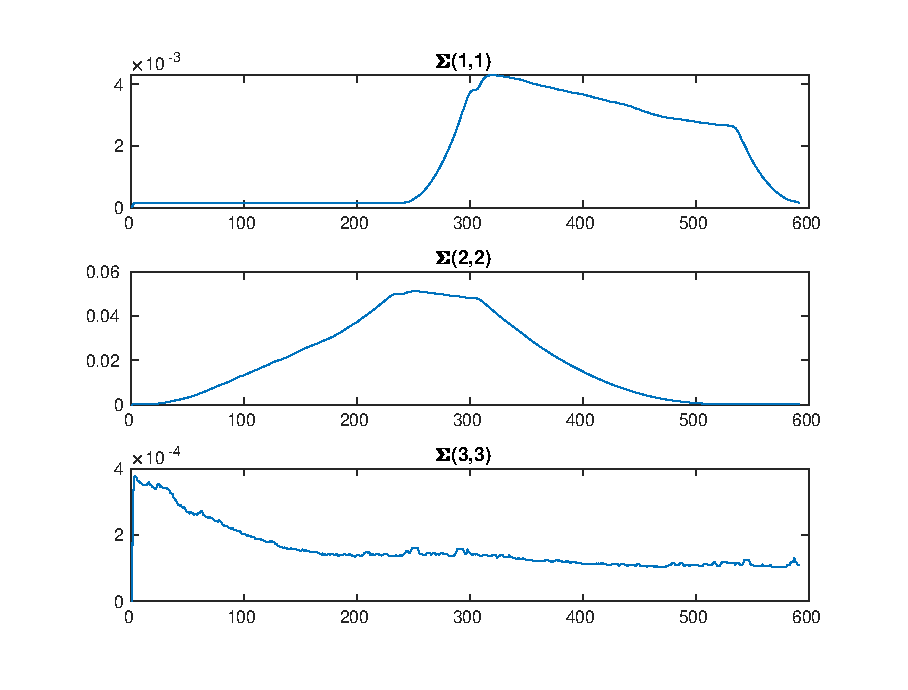
\includegraphics[width=0.45\textwidth]{map_o3+Unknown+Variance.eps}
					\caption{Variance of Robot Pose}
					\label{fig:map_o3+Unknown+Variance}
				\end{figure}
			\par Compared the figures to result of the case of known data association, we could see the unknown data association case could lead to larger error. That might be cause by the affect of landmarks that are not associated with the observation. However, they still need to be considered as a ``weight''. The far away of the landmark from the initial state of the robot, the higher possibility it could deviate from its true position during the operating of the robot.
		\item \texttt{map\_pent\_big\_40.txt} + \texttt{so\_pb\_40\_no.txt}:
			\par The result is illustrated in Fig.~\ref{fig:map_pent_big_40+Unknown+Trace}, \ref{fig:map_pent_big_40+Unknown+Error}, and \ref{fig:map_pent_big_40+Unknown+Variance}. As shown in the figures, the initial part of the EKF-SLAM process acceptable result (which could be seen much clearly on video). However, there appears a sharp changing in orientation of the robot which probably caused by the outlier observation. 
				\begin{figure}[htbp]
					\centering
					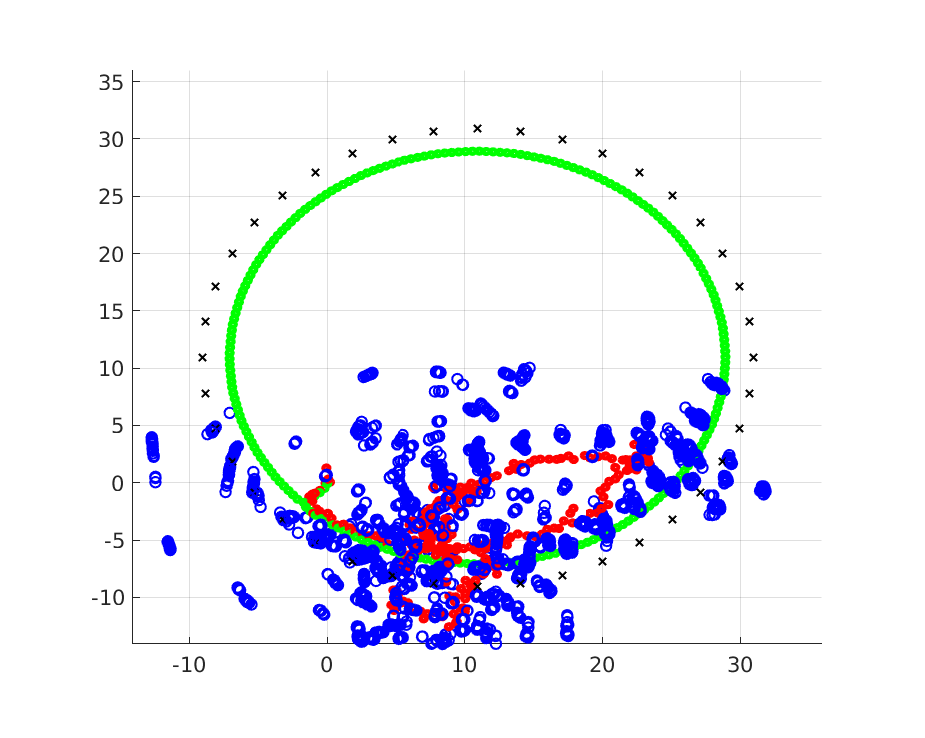
\includegraphics[width=0.45\textwidth]{map_pent_big_40+Unknown+Trace.eps}
					\caption{Trace of Robot Pose and Map Location}
					\label{fig:map_pent_big_40+Unknown+Trace}
				\end{figure}
				\begin{figure}[htbp]
					\centering
					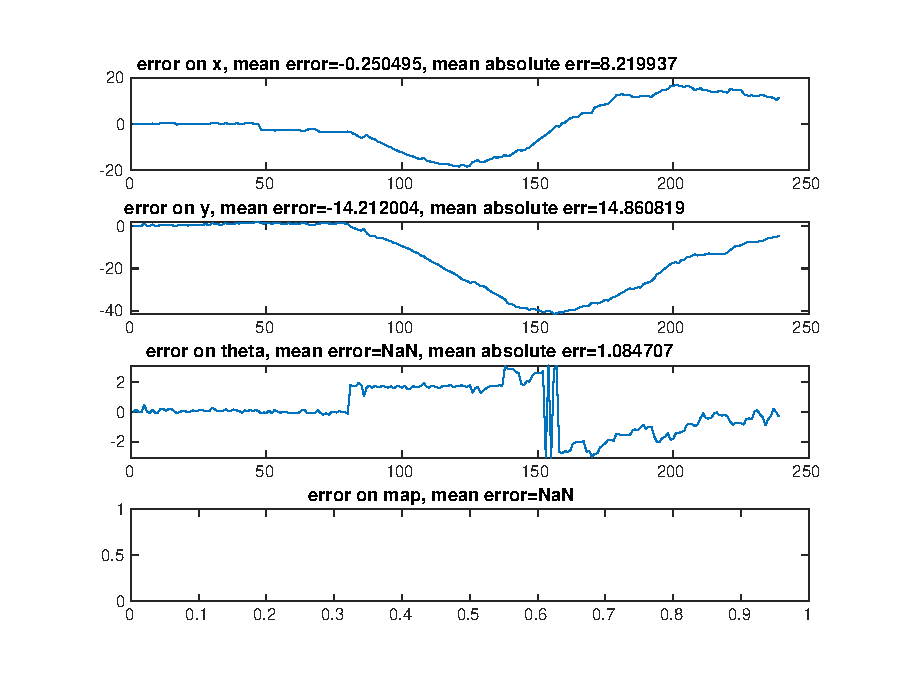
\includegraphics[width=0.45\textwidth]{map_pent_big_40+Unknown+Error.eps}
					\caption{Error of Robot Pose and Average Map Location}
					\label{fig:map_pent_big_40+Unknown+Error}
				\end{figure}
				\begin{figure}[htbp]
					\centering
					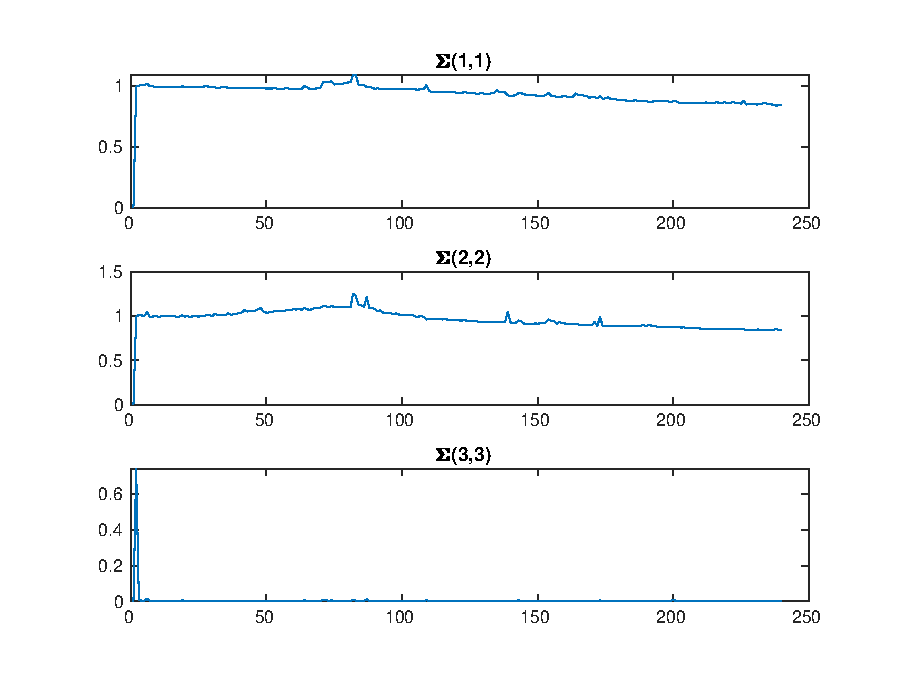
\includegraphics[width=0.45\textwidth]{map_pent_big_40+Unknown+Variance.eps}
					\caption{Error of Robot Pose and Average Map Location}
					\label{fig:map_pent_big_40+Unknown+Variance}
				\end{figure}
	\end{itemize}

%%%%%%%%%% ---------- %%%%%%%%%%
\section{Summary and Conclusions}
\par Extended Kalman filter based Simultaneous  Localization and Mapping is one of the most common solution to SLAM issue and have many applications. In this project, we use MATLAB to implement the algorithm of EKF-SLAM based on the textbook \cite{Probabilistic_Robotics} and simulate the EKF-SLAM with the data sets from \textit{Lab 1}. When implementing the 2-D EKF-SLAM algorithm with unknown data association, we resolve the problem that the algorithm on the textbook have some unclear definition of the size of the matrix.
\par Through the experiment and simulation, we found that the EKF-SLAM can have well performance on relatively well measured data sets which have no or little outlier observation. However, when the data is not precise, the EKF-SLAM would play bad on the estimation of robot pose. Also, wrong data could lead to the wrong new landmarks which means the number of landmarks created in the whole process could larger than the real number of landmarks, and can not be effectively influenced by the change of threshold. Moreover, the EKF-SLAM with unknown data association would have accumulated error because of the inconsistency of the algorithm itself, so after robot has traveled a long journey and comes back to its initial point, it would be difficult for EKF-SLAM to recognize whether the landmark observed is new or not. Based on this point, the EKF-SLAM could have large difficulty on solving the the loop-closure problem.

%%%%%%%%%% ---------- %%%%%%%%%%
\begin{thebibliography}{00}
\bibitem{EKF-SLAM-01} G. Huang, A. Mourikis, and S. Roumeliotis. ``Analysis and Improvement of the Consistency of Extended Kalman Filter Based SLAM,'' \textit{IEEE}, May 2008.
\bibitem{EKF-SLAM-02} J. Castellanos, R. Martinez-Cantin, J. Tardos, and J. Neira, ``Robocentric map joining: Improving the consistency of EKF-SLAM,'' \textit{Robotics and Autonomous Systems}, vol. 55, pp. 21-29, 2007.
\bibitem{SLAM-01} H. Durrant-Whyte, and T. Bailey, ``Simultaneous Localisation and Mapping (SLAM): Part I,'' Jun. 2006.
\bibitem{SLAM-02} T. Bailey, and H. Durrant-Whyte, ``Simultaneous localization and mapping (SLAM): Part II,'' \textit{IEEE Robotics \& Automation Magazine} vol. 13, no. 3, pp. 108-117, Aug. 2006.
\bibitem{Probabilistic_Robotics} S. Thrun, W. Burgard, and D. Fox, ``Probabilistic Robotics,''pp. 309--336, 2005.
\end{thebibliography}
\end{document}
